% Source for the figure of the shortening of the paths (sec. 11.3 and
% 11.4): a path from 0 to its root 5, after find(0) with the compression
% (each node a child of the root) and with the halving (each node of the
% way a child of its grandparent). Build: make figures (in ../build).
\documentclass[border=4pt]{standalone}
\usepackage[T1]{fontenc}
\usepackage{newpxtext,newpxmath}
\usepackage[varqu,varl,scaled=0.95]{zi4}
\usepackage{tikz}
% tikz-ads.tex: the TikZ styles shared by the figures of the memory of the
% manual, \input by each standalone figure: a cell of a vector (cell), the
% cell that an operation touches (touched), a free cell (free), a node of a
% linked structure (node), the labels of indices (index) and of variables
% (var), a pointer (ptr), and \cells and \indices to draw a row of cells.
\usetikzlibrary{arrows.meta,positioning,calc,fit,shapes.multipart}
\definecolor{adsTouched}{RGB}{214,196,236}
\definecolor{adsFree}{RGB}{236,236,236}
\tikzset{
  ads/.style={>={Stealth[length=2mm]},font=\small,
              every node/.append style={inner sep=0pt}},
  cell/.style={draw,minimum width=7mm,minimum height=7mm,
               font=\small\ttfamily,outer sep=0pt},
  touched/.style={cell,fill=adsTouched},
  free/.style={cell,fill=adsFree,text=black!45},
  node/.style={draw,rounded corners=1pt,minimum width=8mm,
               minimum height=6mm,font=\small\ttfamily},
  index/.style={font=\scriptsize\ttfamily,text=black!60},
  var/.style={font=\small\itshape},
  ptr/.style={->,thick}
}
% \cells{name}{x,y}{list}: a row of cells, the first at (x,y), named
% name-0, name-1, ...; each item is text/style, the style one of cell,
% touched and free (e.g., {a/cell,e/touched,/free})
\newcommand{\cells}[3]{%
  \foreach \v/\s [count=\i from 0] in {#3}
    \node[\s] (#1-\i) at ($(#2)+(\i*7mm,0)$) {\v};}
% \indices{name}{n}: the indices 0 .. n-1 under the cells of name
\newcommand{\indices}[2]{%
  \foreach \i in {0,...,\numexpr#2-1\relax}
    \node[index,below=1.2mm of #1-\i] {\i};}

\tikzset{t/.style={circle,draw,minimum size=6mm,font=\small\ttfamily},
  up/.style={->,thick,shorten >=0.5pt}}
\begin{document}
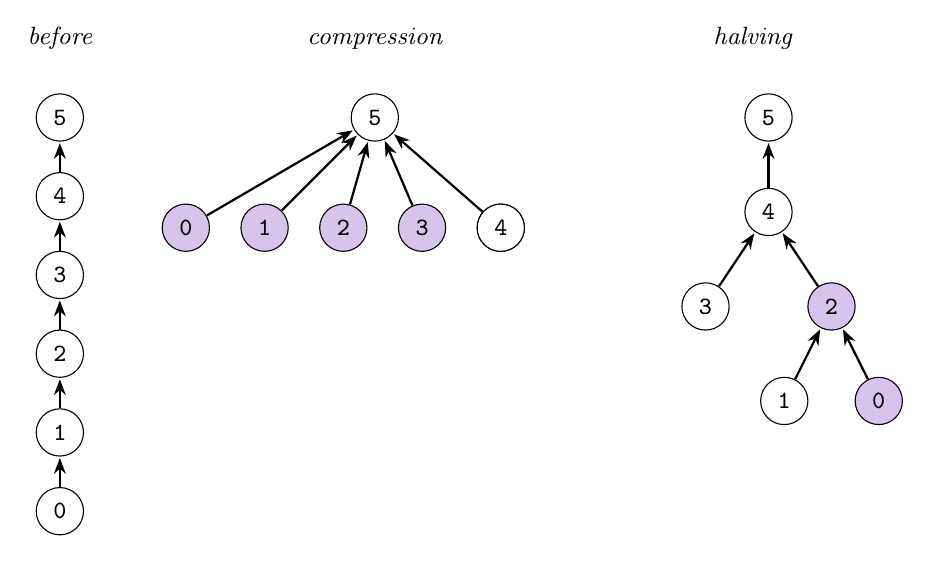
\begin{tikzpicture}[ads]
  % before: a path 0 -> 1 -> 2 -> 3 -> 4 -> 5
  \node[var] at (0,10mm) {before};
  \foreach \i in {0,...,5}
    \node[t] (a\i) at (0,-50mm+\i*10mm) {\i};
  \foreach \i/\j in {0/1,1/2,2/3,3/4,4/5} \draw[up] (a\i) -- (a\j);
  % compression
  \node[var] at (40mm,10mm) {compression};
  \node[t] (c5) at (40mm,0) {5};
  \foreach \i/\x in {0/16,1/26,2/36,3/46,4/56}
    \node[t,fill=adsTouched] (c\i) at (\x mm,-14mm) {\i};
  \node[t,fill=white] at (56mm,-14mm) {4};
  \foreach \i in {0,...,4} \draw[up] (c\i) -- (c5);
  % halving
  \node[var] at (88mm,10mm) {halving};
  \node[t] (h5) at (90mm,0) {5};
  \node[t] (h4) at (90mm,-12mm) {4};
  \node[t] (h3) at (82mm,-24mm) {3}; \node[t,fill=adsTouched] (h2) at (98mm,-24mm) {2};
  \node[t] (h1) at (92mm,-36mm) {1}; \node[t,fill=adsTouched] (h0) at (104mm,-36mm) {0};
  \draw[up] (h4) -- (h5); \draw[up] (h3) -- (h4); \draw[up] (h2) -- (h4);
  \draw[up] (h1) -- (h2); \draw[up] (h0) -- (h2);
\end{tikzpicture}
\end{document}
